\chapter{Аналитическая часть}

\section{Параллелизм}
Параллелизм предполагает выполнения нескольких задач в момент времени. 
Покажем стрелкой зависимость данных, используемых в задаче Б, от данных, используемых в задаче А, как показано на рисунке \ref{fig:picture1.1}.
То есть данные, рассчитанные в результате выполнения задачи А, используются при выполнении задачи Б. 

\begin{figure}[h!]
	\centering
	
\includegraphics[scale=0.4]{img/Связь.png}
	\caption{Зависимость задачи А от задачи Б по данным}
	\label{fig:picture1.1}
\end{figure}

Выделяют два вида параллелизма \cite{paralleltype}: конечный, когда можно параллельно выполнять отдельные инструменты или их набор, и массовый, предполагающий параллельное исполнение итераций циклов. 
В свою очередь массовый параллелизм делится еще на два: покоординатный -- вычисления в пределах одной координаты не зависят по данным от вычислений для другого значения координаты, и скошенный. 
Зависимость по данным задач представлена на рисунке \ref{fig:picture1.2}.

\begin{figure}[h!]
	\centering
	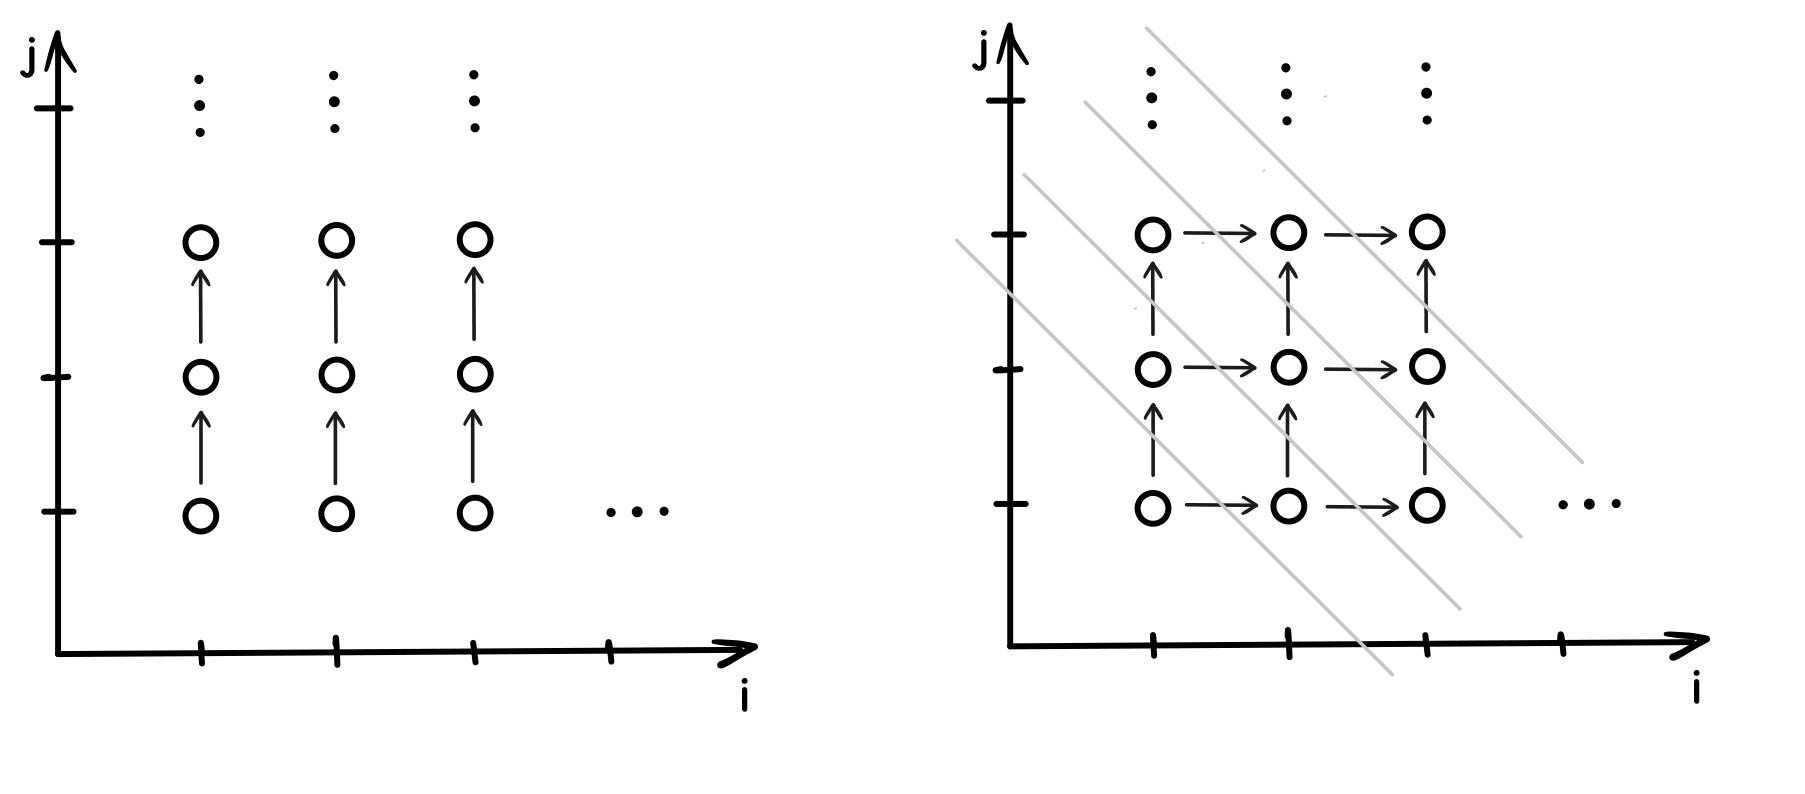
\includegraphics[scale=0.9]{img/Параллелизм.png}
	\caption{Покоординатный и скошенный параллелизм}
	\label{fig:picture1.2}.
\end{figure}

\section{Блочная сортировка}

Блочная сортировка \cite{bucket} -- это алгоритм сортировки, который разделяет несортированные элементы массива на несколько групп, называемых блоками или \textbf{корзинами}. 
Затем каждая корзина сортируется с использованием любого из подходящих алгоритмов сортировки или рекурсивного применения того же алгоритма блочной сортировки. 

Мной были найдены реализации данной сортировки только для положительных чисел, поэтому этап поиска интервала -- размера блока был усовершенствован, дабы алгоритм был применим и для отрицательных чисел. 

В итоге отсортированные сегменты объединяются для формирования окончательного отсортированного массива.

Исходя из общей концепции, алгоритм может быть разбит на следующие части: 
\begin{itemize}
	\item определение числового интервала -- объема блока;
	\item распределение чисел массива по корзинам;
	\item сортировка каждого отдельного блока.
\end{itemize}

Последний пункт является циклом, на каждой итерации которого рассматривается отдельная корзина: то есть данные и операции над ними на одной итерации цикла не влияют на данные на другой. 
Таким образом этот этап алгоритма сортировки может быть реализован с помощью распараллеливания -- покоординатный вид массового параллелизма. 

\section{Вывод}

В данном разделе были рассмотрены основополагающие материалы, которые в дальнейшем потребуются при параллельной и однопоточной реализации алгоритма блочной сортировки.

